%%%%%%%%%%%%%%%%%%%%%%%%%%%%%%%%%%%%%%%%%%%%%%%%%%%%%%%%%%%%%%%%%%%%%%%%%%%%%%%%%%
%%%  ISWC 2016 Demo: Exploring Linked Classical Music Catalogs with OVERTURE  %%%%
%%%%%%%%%%%%%%%%%%%%%%%%%%%%%%%%%%%%%%%%%%%%%%%%%%%%%%%%%%%%%%%%%%%%%%%%%%%%%%%%%%

\documentclass[runningheads,a4paper]{llncs}
\usepackage{graphicx}
\usepackage{amsmath}
\usepackage{todonotes}
\usepackage{hyperref}
\usepackage{amssymb, bm}
\usepackage{indentfirst}

%%%%%%%%%%%%%%%%%%%%%%%%%%%%%%%
%%%  Beginning of document  %%%
%%%%%%%%%%%%%%%%%%%%%%%%%%%%%%%

\begin{document}

\title{Exploring Linked Classical Music Catalogs\\ with OVERTURE}
\titlerunning{Exploring Linked Classical Music Catalogs with OVERTURE}

\author{Pasquale Lisena$^1$, Manel Achichi$^2$, Eva Fern\'{a}ndez$^1$, \\ Konstantin Todorov$^2$, Rapha\"{e}l Troncy$^1$}
\authorrunning{Lisena \textit{et al.}}
\institute{$^1$EURECOM, Sophia Antipolis, France\\$^2$University of Montpellier, France}

\maketitle

%%%%%%%%%%%%%%%%%%
%%%  Abstract  %%%
%%%%%%%%%%%%%%%%%%

\begin{abstract}
In this paper, we introduce OVERTURE---a web application allowing to explore the interlinked catalogs of major music libraries including the French National Library, Radio France and the Philharmonie de Paris. We have first developed the DOREMUS ontology which is an extension of the well-known FRBRoo model for describing works and expressions as well as the creation process. We have implemented a so-called \textsc{marc2rdf} tool allowing for the conversion and linking of bibliographical entries about music works, interpretations and expressions from their original MARC-format to RDF following this DOREMUS ontology. We present an exploratory search engine prototype that enables to browse through the reconciled collection of bibliographical records of classical music and to highlight the various interpretations of a work, its derivative, its performance casting as well as other rich metadata.
\end{abstract}

%%%%%%%%%%%%%%%%%%%%%%%%%%%%%%%%%%%%%%%%%%%%%%%%%%%%%
%%%  1. From Music Metadata to Linked RDF Graphs  %%%
%%%%%%%%%%%%%%%%%%%%%%%%%%%%%%%%%%%%%%%%%%%%%%%%%%%%%

\section{From Music Metadata to Linked RDF Graphs}
\label{sec:conversion}
The DOREMUS project\footnote{\url{http://www.doremus.org/}} develops methods to describe, publish, connect and contextualize music catalogs on the web of data. Our focus is on the description of classical and traditional musical works as well as their interpretations (events)~\cite{achichi2015doremus}. We rely therefore on the FRBRoo model, which combines the strength of the FRBR practices in distinguishing a work from its interpretation and derivatives and the CIDOC-CRM model that emphasizes the role of events for modeling the process of creation of creative works. We extend FRBRoo by adding classes and properties specific to the music domain (e.g. for representing the intended casting for interpreting a work). The research challenges we are tackling are related to the population of this rich ontological model from raw library metadata and on its visualization that should enable users to search for classical music but also see influencers and derivative works, or the many interpretations of a famous work.

\paragraph{{\bf Data Conversion.}} The data collected from the BnF and the Philharmonie de Paris (PP) describing music works are represented in the MARC format (UNI-- and INTERMARC variants). A MARC file is a succession of fields, each carrying a 3-digit label, and subfields, delimited by the \$ symbol (Fig.~\ref{fig:unimarc}). The semantics of these fields and subfields is described in documents issued by The International Federation of Library Associations and Institutions (IFLA)\footnote{\url{http://www.ifla.org/publications/ifla-series-on-bibliographic-control-36}.}. Note that a subfield tag can change its meaning depending on the field, under which it is found. In our example (Fig.~\ref{fig:unimarc}), the \$a tag under the field 500 stands for the musical genre (sonata), whereas the same tag under the field 700 stands for the composer name (Beethoven). We have developed an open source prototype that allows for the automatic conversion of UNI- or INTERMARC bibliographic records to RDF\footnote{\url{https://github.com/DOREMUS-ANR/marc2rdf}}, implementing the DOREMUS model~\cite{choffe2016doremus}. The conversion process relies on explicit expert-defined transfer rules (or mappings) that indicate where in the MARC file to look for what kind of information, providing the corresponding property path in the model as well as useful examples that illustrate each transfer rule, as shown in Fig.~\ref{fig:mappings}. We have used the DOREMUS properties to name the extracted relations (e.g., \texttt{mus:U12$\_$has$\_$genre}\footnote{The \texttt{mus} prefix refers to \url{http://data.doremus.org/ontology/}} is the property describing the genre of a work). Resources are identified by URIs that use the corresponding DOREMUS class labels in their names (as for example \url{http://data/doremus.org/expression/UUID} identifying an instance of the FRBRoo class \texttt{Expression}).
\begin{figure}
  \centering
  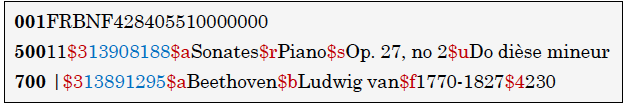
\includegraphics[width=6cm]{img/marc-exmpl-simple.png}
  \caption{An excerpt of a UNIMARC record.}
  \label{fig:unimarc}
%\end{figure}
\smallskip
%\begin{figure}
  \centering
  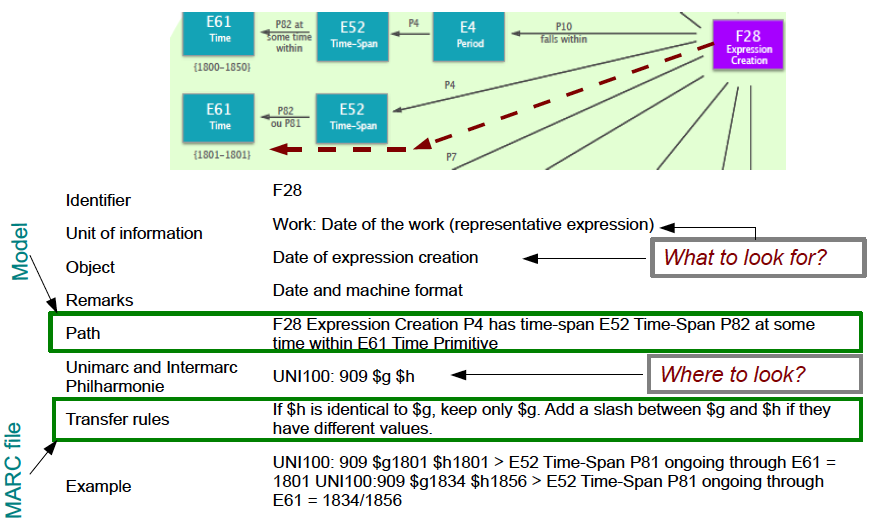
\includegraphics[width=8cm]{img/mapping-rules.png}
  \caption{Example of mapping rules describing the timespan of the composition of a work.}
  \label{fig:mappings}
\end{figure}
\vspace{-0.5cm}
Often, the RDF data that we extract will contain string literals, such as genres ({\it sonata}) or instruments ({\it piano}). These values are controlled by specific vocabularies, such as MIMO\footnote{\url{http://www.mimo-international.com/vocabulary.html}} describing musical instruments. Therefore, our data conversion methods include an automatic mapping of string literals to URIs coming from controlled vocabularies. Inspired by the Datalift platform~\cite{datalift}, we have developed a generic \texttt{string2uri} component enabling to lookup strings in a SKOS controlled vocabulary and to propose best candidate match.

Among the several existing MARC to RDF conversion tools, such as the Catamandu toolkit\footnote{\url{http://librecat.org}} or \textsc{marcmods2rdf}\footnote{\url{http://simile.mit.edu/repository/RDFizers/marcmods2rdf/}}, the one that is closest in spirit to ours is Marimba\footnote{\url{http://marimba4lib.com}}, developed in the context of the Linked Data at the BNE (Biblioteca Nacional de Espa\~na) project. Just like our converter, and in contrast to Catmandu and \textsc{marcmods2rdf}, Marimba is based on the IFLA ontologies, including FRBR, and is designed by the help of librarians. However, Marimba focuses on literature library entries, while we implement the DOREMUS model, which is better suited to describe music.

\paragraph{{\bf Data Heterogeneities and Linking.}} Due to the high data heterogeneity, link discovery in the musical field becomes a challenging task. To train and test data linking tools, we have collected benchmark data from the BnF and the PP, now part of the OAEI instance matching evaluation campagne\footnote{\url{http://islab.di.unimi.it/content/im_oaei/2016/\#doremus}}. Our tests with SILK~\cite{jentzsch2010silk} and LIMES~\cite{ngomo2011limes}, achieving an average F-measure of around 55\%, confirm that new methods, specific to the music field, need to be proposed, in order to handle specific heterogeneity types of these datasets. In particular, special attention has to be payed to multilingual descriptions of works, as well as to significant lexical differences in work titles. Descriptive heterogeneities (level of detail, number of properties) also hinder the performance of general purpose tools. Furthermore, certain properties, although mapped correctly according to the transfer rules, contain highly heterogeneous information, as for example \texttt{cidoc-crm:P3$\_$has$\_$note} -- a field of free text in the form of comments. We are currently developing a linking approach that combines expert heuristics with indexing techniques that is able to propose a solution according to the heterogeneity type manifested by the data.

%%%%%%%%%%%%%%%%%%%%%%%%%%%%%%%%%%%%%%%%%%%%%%%%%%%%%%%%%%%%%
%%%  2. OVERTURE: an Exploratory Search Engine for Music  %%%
%%%%%%%%%%%%%%%%%%%%%%%%%%%%%%%%%%%%%%%%%%%%%%%%%%%%%%%%%%%%%

\section{OVERTURE: an Exploratory Search Engine for Music}
\label{sec:overture}
%\begin{figure}
%  \centering
%  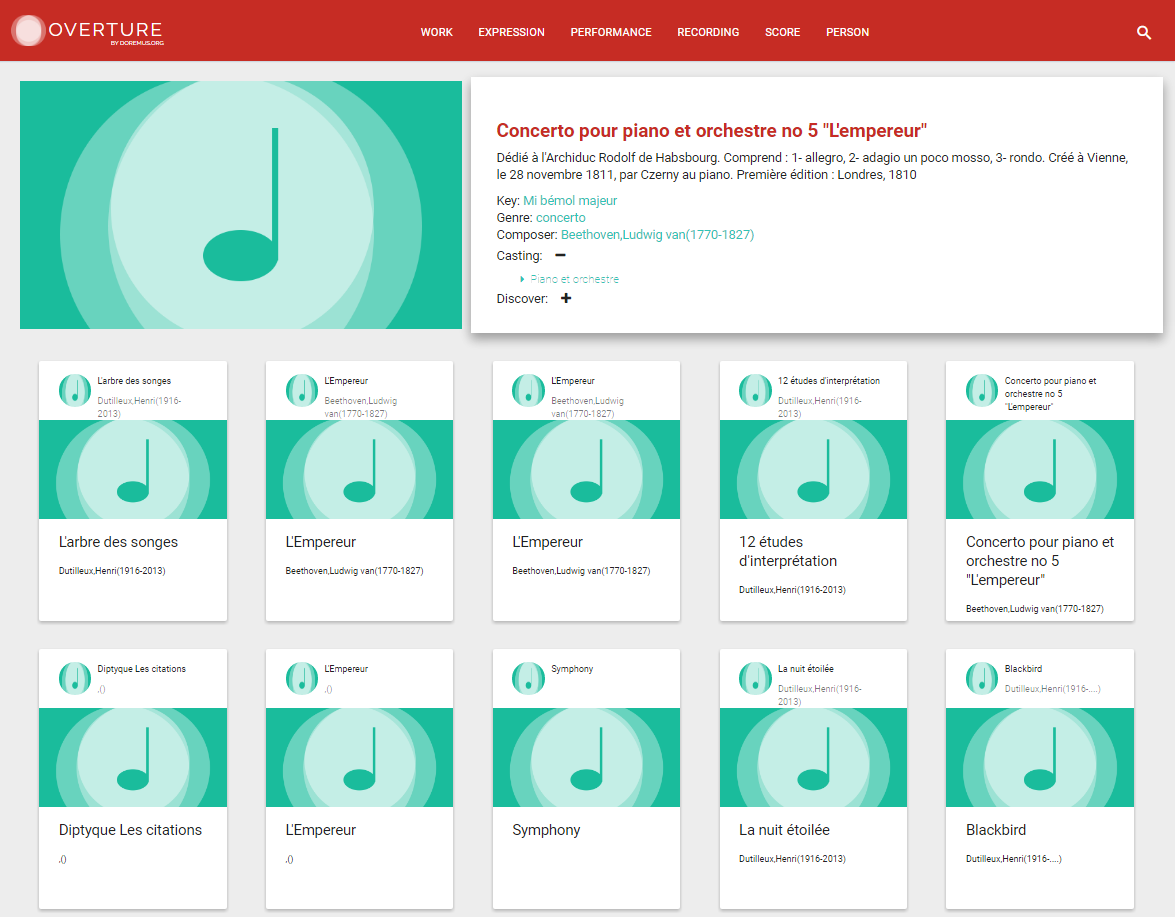
\includegraphics[width=10cm]{img/overture-detail.png}
%  \caption{Overture: browsing a particular interpretation of the Piano Concerto No. 5 from Beethoven}
%  \label{fig:overture-detail}
%\end{figure}

OVERTURE (Ontology-driVen Exploration and Recommendation of mUsical REcords) is a modern web application that relies on a Node.JS server sitting in front of a Virtuoso triple store. The web application performs SPARQL queries to access the data via the Node.JS server that could be a Linked Data Fragment server. The user interface is realized with the AngularJS2 library. At the top, a navigation bar directs the user towards one of the main concepts in the DOREMUS model (Work, Expression, Performance, Recording, Score, Person), that become distinct sections of the application. Inside each section, the user can filter the list of records shown in a class-specific and advanced search form. In this way, (s)he can search a performance by choosing a particular location, a performer, or an expression by selecting the musical key, the genre or by searching by title. From these parameters, the server generates the SPARQL query that matches the user information need.

\begin{verbatim}
SELECT ?expressions ?title
WHERE {
   ?expressions a frbroo:F22_Self-Contained_Expression ;
     cidoc:P102_has_title ?title .
     mus:U12_has_genre <http://data.doremus.org/vocabulary/genre/si>
}
\end{verbatim}

Clicking on a result, more detailed information is shown such as the information about the composer, the casting, a longer descriptive note or different expressions. In the future, this selection will contain related expressions, selected through a recommendation algorithm. The application is available at \url{http://overture.doremus.org}\footnote{A video is also available at \url{https://www.dropbox.com/s/4e7n5a4qgyzk6wu/OvertureDemo-v0.mp4?dl=0}}.

\section*{Acknowledgments}
This work has been partially supported by the French National Research Agency (ANR) within the DOREMUS Project, under grant number ANR-14-CE24-0020.

\bibliographystyle{abbrv}
\bibliography{bib-doremus}

\end{document}
